\documentclass[8 pt]{article}

\usepackage[utf8x]{inputenc}
\usepackage{dsfont}
\usepackage{amsthm}
\usepackage{amsfonts}
\usepackage{amssymb}
\usepackage{tensor}
\usepackage{mathtools}
\usepackage[T1]{fontenc}
%\usepackage[spanish]{babel}
\usepackage[cm]{fullpage}
\usepackage{graphicx}
%\usepackage{float}
\usepackage{bm}
\usepackage{setspace}
\usepackage{enumitem}
\usepackage{mdwlist}
\usepackage{parskip}
\usepackage{listings}
\usepackage{color}
%\usepackage{epstopdf}
\usepackage{tikz,datatool}
\usepackage{hyperref}
\usepackage{mathabx}
\usepackage{multicol}
\usepackage{caption}

\newcommand{\HRule}{\rule{\linewidth}{0.5mm}}

\AtBeginDocument{
  \let\myThePage\thepage
  \renewcommand{\thepage}{\oldstylenums{\myThePage}}
}

\newcommand{\gra}{$^\text{o}$}
\newcommand{\dif}{\text{d}}
\newcommand{\avg}[1]{\left\langle #1 \right\rangle}
\newcommand{\ket}[1]{\left| #1 \right\rangle}
\newcommand{\bra}[1]{\left\langle #1 \right|}
\newcommand{\bket}[2]{\left\langle #1 \middle| #2 \right\rangle}
\newcommand{\der}[2]{\frac{\text{d} #1}{\text{d} #2}}
\newcommand{\prt}[2]{\frac{\partial #1}{\partial #2}}
\newcommand{\dert}[3]{\frac{\text{d}^#3 #1}{\text{d} #2^#3}}
\newcommand{\prtt}[3]{\frac{\partial^#3 #1}{\partial #2^#3}}
\newcommand{\dl}{\mathcal{L}}
\newcommand{\dha}{\mathcal{H}}
\newcommand{\vol}{\text{vol}}
\renewcommand{\vec}[1]{\pmb{#1}}

\DeclarePairedDelimiter\ceil{\lceil}{\rceil}
\DeclarePairedDelimiter\floor{\lfloor}{\rfloor}

\newenvironment{Figure}
  {\par\medskip\noindent\minipage{\linewidth}}
  {\endminipage\par\medskip}

\begin{document}

\begin{minipage}{\textwidth}
    \centering
    \Large \textbf{\textsc{Homework 1: An option's fair price}}\\[0.5cm]

    \small \textsc{Francisco García Flórez, Joris van Lammeren, Wouter Varenkamp}\\[0.5cm]

    \begin{minipage}{0.6\textwidth}
      \textbf{Abstract.} In this first homework we will be computing using a Monte Carlo method the exercise value of a share, which we will then use to determine a fair price for a call option of that share.
    \end{minipage}
\end{minipage}

\section{Computing the share's value via a Wiener process}

Firstly, we need to compute the value of the share itself after a certain amount of time. For this purpose we will solve the following stochastic differential equation, known as \emph{Wiener process} \cite{Wilmott}:

\begin{equation}
  \frac{\dif S}{S} = \sigma \dif X + \mu \dif t ~~~ ,
\end{equation}

where $\sigma$ is the volatility, $\mu$ is the drift and $S(t)$ the value of the option as a function of time. Instead of solving it analytically, we can discretize it as in \cite{sde} to find

\begin{equation}
  S_{i+1} = S_i \left( 1 + \sigma \Delta W_i + \mu \Delta t_i \right) ~~~ ,
\end{equation}

where $\Delta W_i = \sqrt{\Delta t_i} N(0, 1)$, simulating the random walk. In our case the time step is constant, so every $\Delta t_i$ will have the same value. The value after $nt$ time steps is the value at expiration date, which we will use to determine the price of the option.

\section{Determining fair prices for call options}

Now that we can compute the exercise value of the share, we can use it to determine how much we can pay for a call option for that share. Since this is not a value that can be derived via an objective procedure, we will consider two approaches to compute the price: the \emph{risk-free approach} and the \emph{risky approach}.

\subsection{Risk-free approach}

For the \textbf{risk-free approach}, we consider the probability distribution of the value of the share at expiration date, which will be a normal $N(\mu, \sigma)$. Now, since buying the call option gives us the \emph{right} to buy the share at the exercise price, we can choose not to use it if that means losing money. To represent this fact, instead of using the previous normal for our computations, we take every instance with share price lower than the exercise price and assign a profit of zero to it, instead of a negative value.

In the following plots we can clearly see that transformation:

\begin{center}
  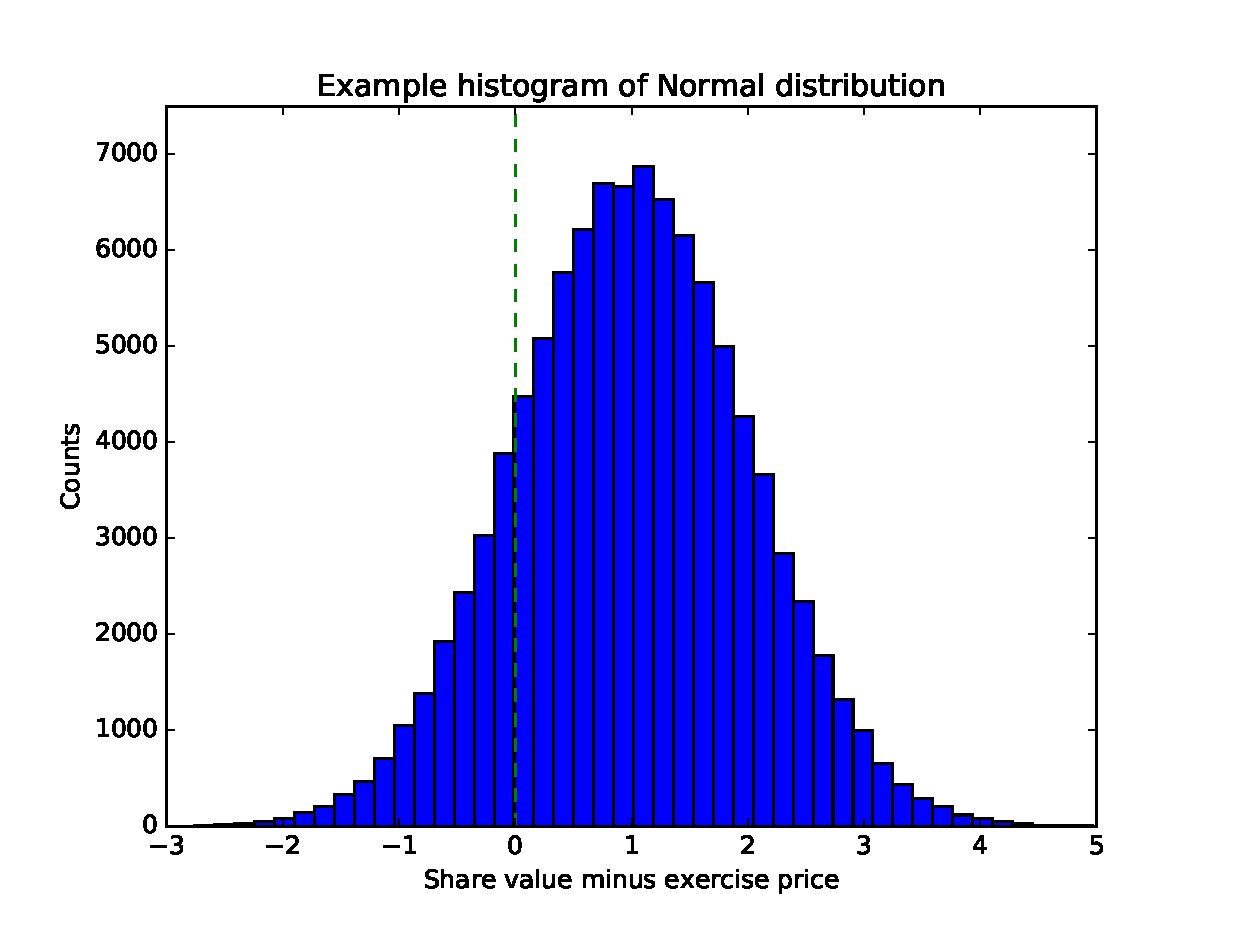
\includegraphics[width=0.45\textwidth]{graphs/ex-normal-1.eps}
  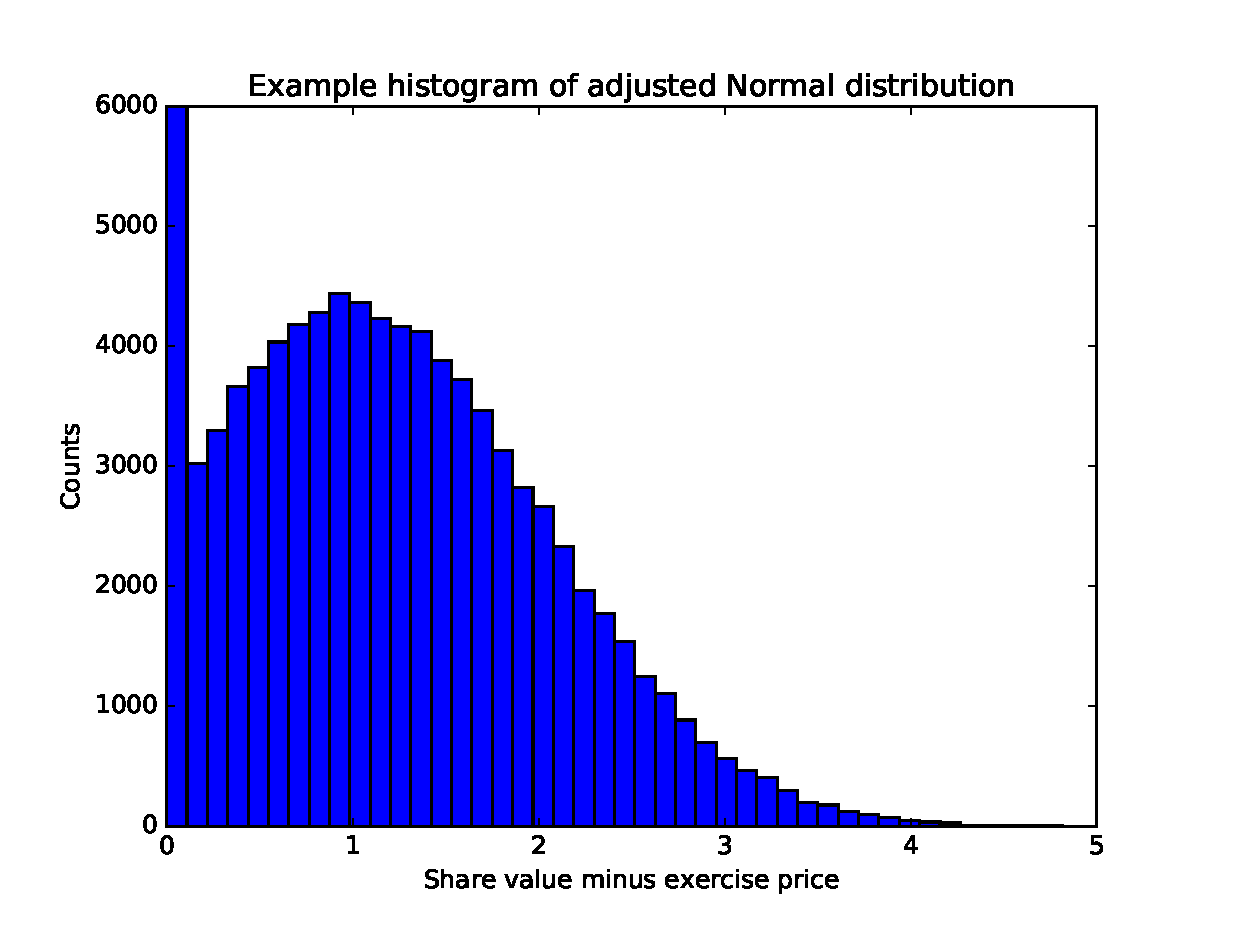
\includegraphics[width=0.45\textwidth]{graphs/ex-normal-2.eps}
\end{center}

Using this new probability distribution we can compute the risk-free price as the \textbf{average value} of it. This price is the minimum profit that on average we expect to make, so the fair price using this approach would be any amount smaller than the sum of the exercise price plus this value, as much as the writer of the option is willing to accept.

We can write this as

\begin{equation}
  \avg{oP}_{rf} \equiv \avg{\tilde N(\mu, \sigma)} ~~~ ,
\end{equation}

where $\avg{oP}_{rf}$ is the option price computed risk-free, and $\tilde N(\mu, \sigma)$ is the adjusted normal distribution.

\subsection{Risky approach}

On the other hand, we can take a \textbf{risky approach} and pay more than the risk-free price with a smaller probability of having profits. For this to be quantitative we have to assign a risk value to a price, in a way that zero corresponds to making the average profit and one corresponds to the impossible case of having profit paying an infinite amount of money.

So, assuming the expiry values of the share is a random variable with normal distribution, we can introduce the risk as a value $P \in [0, 1)$ and compute the probability of making average profit using the cumulative distribution function (cdf) as

\begin{equation*}
  \text{cdf}(\avg{oP}_{rf}, \mu, \sigma) ~~~ ,
\end{equation*}

and then computing the final probability using $P$ as

\begin{equation*}
  \text{cdf}(\avg{oP}_{rf}, \mu, \sigma)(1 - P) + P ~~~ .
\end{equation*}

Now, what we are doing here is mapping the interval $[\text{cdf}(\avg{oP}_{rf}, \mu, \sigma), 1)$ to $[0, 1)$, so that computing now the inverse cdf of this probability we can map the expected profits interval, $[\avg{oP}_{rf}, \infty)$, to $P \in [0, 1)$. We can write this calculation as

\begin{equation}
  \avg{oP}_r \equiv \text{cdf}^{-1} \left( \text{cdf}(\avg{oP}_{rf}, \mu, \sigma)(1 - P) + P \right) ~~~ .
\end{equation}

\section{Results}



\begin{thebibliography}{28}
\raggedright
\addcontentsline{toc}{section}{Bibliography}

\bibitem{Wilmott} P. Wilmott et al, \emph{The Mathematics of Financial Derivatives}, 1995.

\bibitem{sde} Timothy Sauer, \emph{Handbook of Computational Statistics}, Springer, pp 529-550, July 2011.

\end{thebibliography}

\end{document}
